\documentclass[10pt, letterpaper, answer]{exam}
\usepackage{graphicx, amsmath, url, tikz, hyperref}   
\usepackage[margin=1in]{geometry}
\usetikzlibrary{decorations.pathreplacing}


% Comment this out to remove answer boxes.
\printanswers


\begin{document}
\begin{center}
{\Large Thermohaline Circulation} \\ \vspace{1cm} UBC Math 215/255, 2024WT1. S.~Bachmann \& K.~Dao Duc \\
P.~Harrington and N.~Bailey
\end{center}


\section{The Stommel model}

Oceanic currents are central to the regulation the Earth's climate. Two key drivers of oceanic currents are differences in temperature and salinity (concentration of salt) between high and low latitudes. Increased melting
of ice and increased precipitation at the poles, as well as increased evaporation at in the tropics, caused by climate change perturbs this circulation pathway on very slow timescale.

The goal of this assignment is to explore the behaviour of this dynamical system and to understand how a small change in the melting of ice in the polar regions can cause a drastic change the oceanic currents. 

\begin{figure}[h]
    \centering
    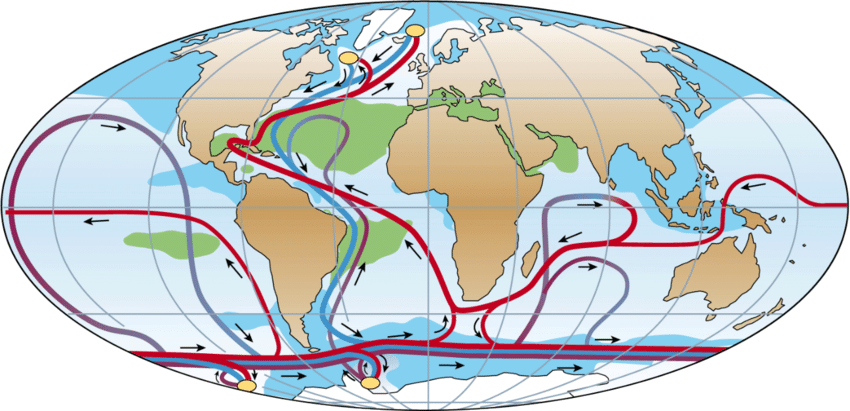
\includegraphics[width=0.4\linewidth]{Simplified-sketch-of-the-global-thermohaline-circulation-pathway-whereby-yellow-dots.png}
    %\caption{Simplified Sketch of the Global Thermohaline Circulation Pathway (Rahmstorf)}
    \label{fig:enter-label}
\end{figure}

The \emph{Stommel model} reduces the Northern Atlantic ocean to two boxes representing respectively the high-latitude (polar) region and low-latitude (tropical) region. Each of them has its own water temperature and water salinity, and there is a surface flow $q$ as pictured below:
\begin{figure}[h]
\centering
    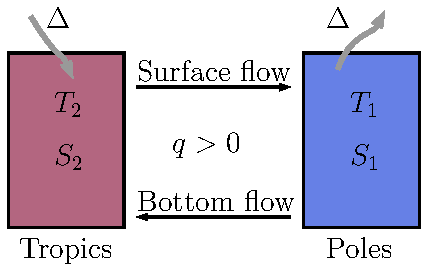
\includegraphics[width = 0.3\linewidth]{Stommel.pdf}
    \caption{The two-vessel model. The relevant parameters are the differences $T_2 - T_1$ and $S_2 - S_1$. An influx of fresh water at the poles corresponds to a decrease in salinity, represented by $\Delta$.}
    \label{fig:enter-label}
\end{figure}
When $q>0$ the flow of water on the bottom of the ocean is from high latitudes to low latitudes, which creates an equal flow on the surface of the ocean from low latitudes to high latitudes.

The flow of water $q$ depends on the differences $T_2 - T_1$ and $S_2 - S_1$ (which is itself influenced by the flux~$\Delta$) and it can be modelled by the equation
\begin{equation}
    \frac{dq}{dt} = -|q|(q - k_1) - k_2,
\end{equation}
where the positive constant $k_1$ is proportional to the difference $T_2 - T_1$ in temperature between high and low latitudes and the positive constant $k_2$ depends on $\Delta$. The key to this assignment is that \emph{an increase in glacial melting will increase $k_2$}, and we shall explore the consequences of this fact.

%%%%%%%%%%%%%%%%%%%%%%%%%%%%%%
\section{Qualitative analysis}
\begin{enumerate}
    \item Find the steady state solutions for $q$. You should consider the case where $q>0$ and the case where $q<0$ separately.  You should be able to disregard one of the solutions you find in one of the cases because of a contradiction. 

    \item Let us fix the value of $k_1$. Under which condition do steady states with $q\geq0$ exist?

\item Determine the stability of the steady states. To simplify notations, you can call $k_c = \frac{k_1^2}{4}$.



\item The North Atlantic current has been such that $q>0$ for thousands of years. Describe this situation in terms of your findings above.



\item Assume now that because of increased glacial melting, a large amount of freshwater flows into the polar ocean. Based again on your analysis above, explain what could happen to the current.

 
\end{enumerate}

%%%%%%%%%%%%%%%%%%%%%%%%%%%%%%
\section{Slope field}
Below are two plots of the slope field (for $t>0$) associated with the equation:
\begin{center}
\begin{minipage}{0.75\linewidth}
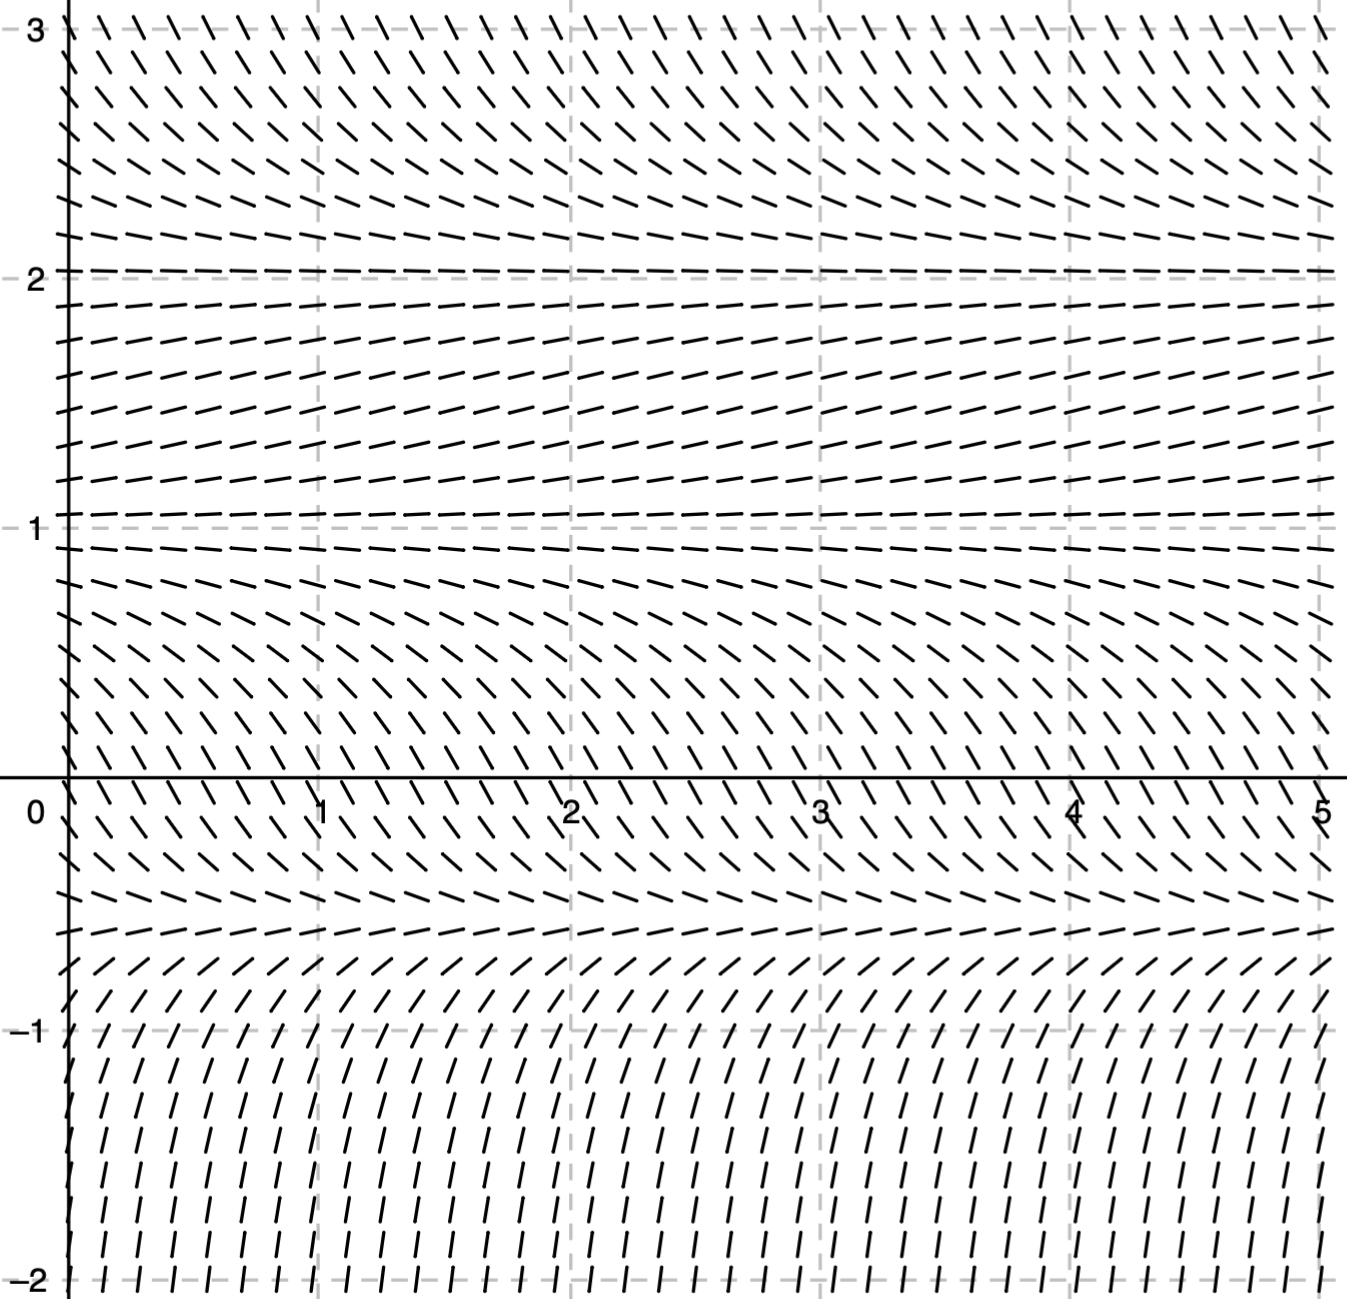
\includegraphics[width=0.35\linewidth]{Field_1} 
    %\caption{Vlieger}
    \hfill
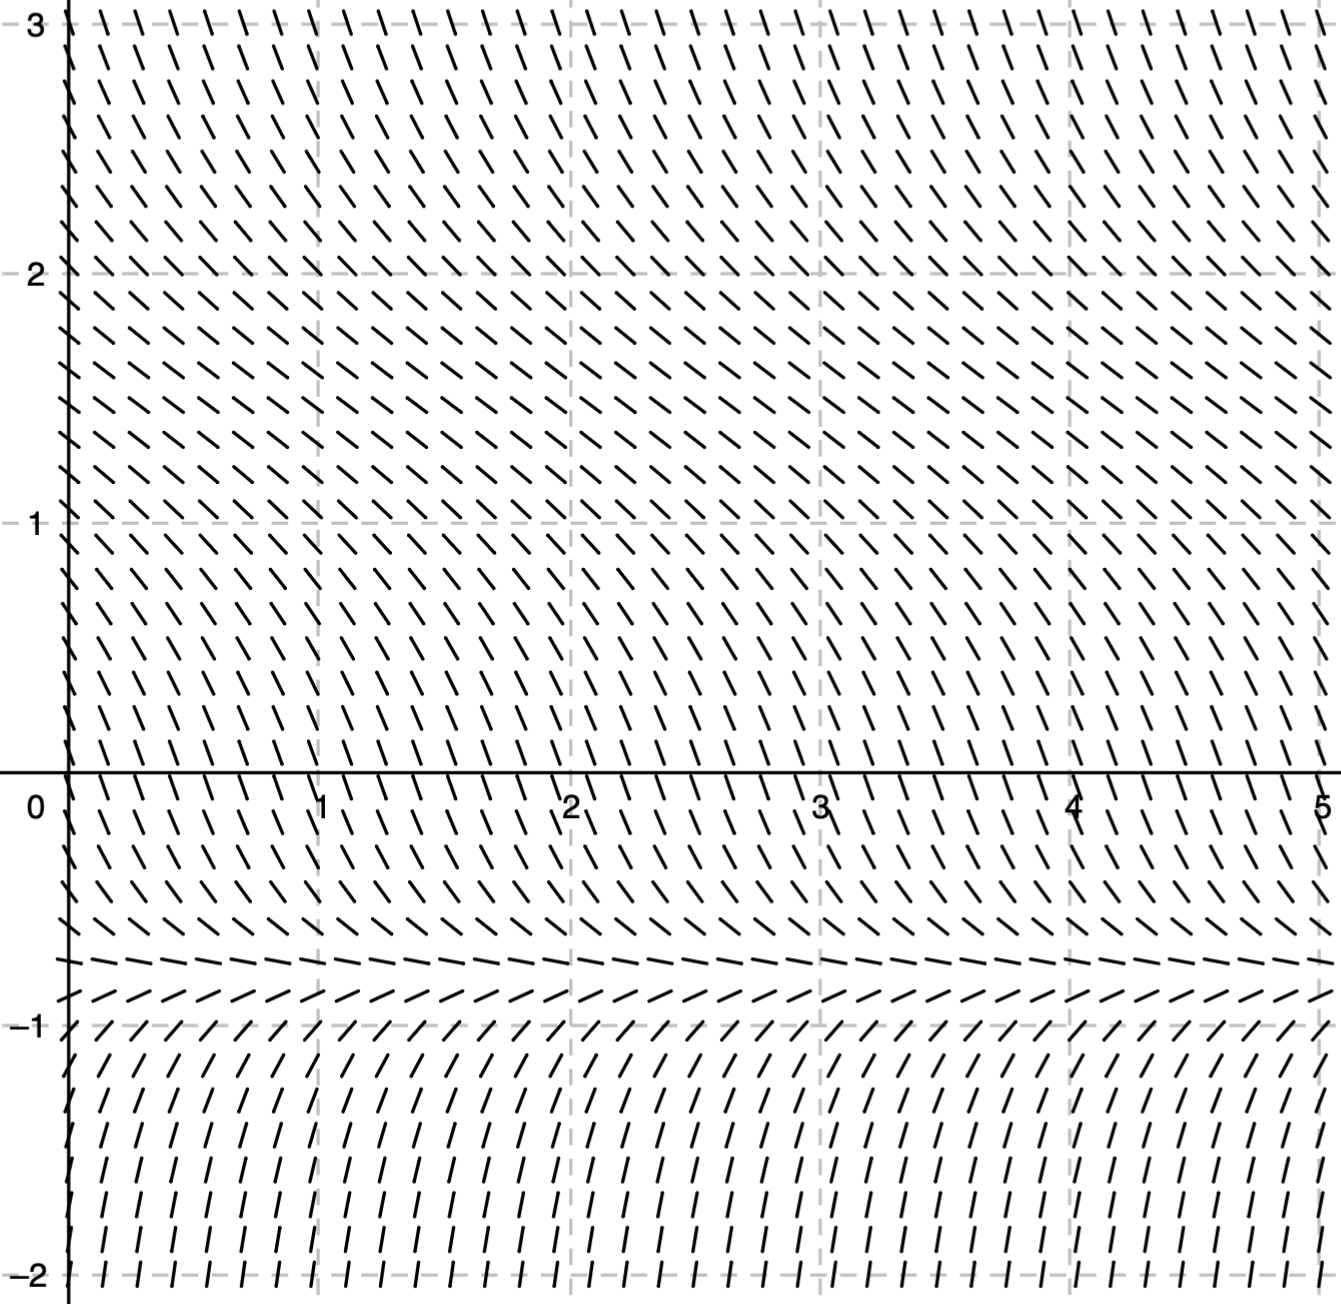
\includegraphics[width=0.35\linewidth]{Field_2}
\end{minipage}
\end{center}
In each case, determine whether $k_2<k_c$ or $k_2>k_c$ and draw a few integral curves (solutions).



%%%%%%%%%%%%%%%%%%%%%%%%%%%%%%
\section{Analytical solution}
We can actually solve the initial value problem explicitly:
\begin{equation}
    \dfrac{dq}{dt} = -|q|(q - k_1) - k_2, \quad q(0)=q_0.\label{eq:q}
\end{equation}
We will do that here in the case $k_2<k_c$.
\begin{enumerate}
\item Assume first that $q_0>0$. Solve~(\ref{eq:q}) and denote the solution $q^+(t)$. 

\item What is the asymptotic behaviour $t\to+\infty$ of your solution in the case $q_0\geq q_2^+$? Does it match with the phase line analysis in the previous section?

\item Let now $0<q_0<q_2^+$. What does the phase line analysis predict? Check the validity of this prediction with the exact solution.




\item The case $q_0<0$ can be treated along very similar lines, with the solution given by
%
\begin{equation*}
q^-(t)  = \frac{(q^-_2-q_0)q^-_1 - (q^-_1-q_0)q^-_2 \mathrm{e}^{(q^-_1-q^-_2)t}}{(q^-_2-q_0)-(q^-_1-q_0)\mathrm{e}^{(q^-_1-q^-_2)t}}.
\end{equation*}
%
Here we denoted $q^-_2 = q^-$ while $q^-_1$ is the discarded solution in Question~1 of the previous section. Analyse again the asymptotic behavious of your solution.


\item (a) Describe the complete behaviour of the solution in the case $0<q_0<q_2^+$ using the conclusions of 3,4 above. What does your finding mean for the oceanic flow?

(b) Construct explicitly a continuous solutions $q(t)$ that changes sign at $t_*$.
%


\end{enumerate}

\vspace*{\fill}

\noindent If you feel overwhelmed by the climate emergency, support can be found here: \\
\url{https://climateemergency.ubc.ca/stem-and-climate-wellbeing-toolkit/}

\end{document}